\documentclass{scrartcl}
\usepackage{xcolor, tikz}
\usepackage{pgfplots}
\pgfplotsset{compat=newest}
\pagestyle{empty}
\definecolor{pdg2112}{RGB}{228,26,28}
\definecolor{pdg2212}{RGB}{55,126,184}
\definecolor{pdg1000010020}{RGB}{153,153,153}
\definecolor{pdg1000020040}{RGB}{166,86,40}
\definecolor{pdg11}{RGB}{152,78,163}
\definecolor{pdg1000060110}{RGB}{153,153,153}
\definecolor{pdg22}{RGB}{77,175,74}
\definecolor{pdg1000060120}{RGB}{153,153,153}
\begin{document}
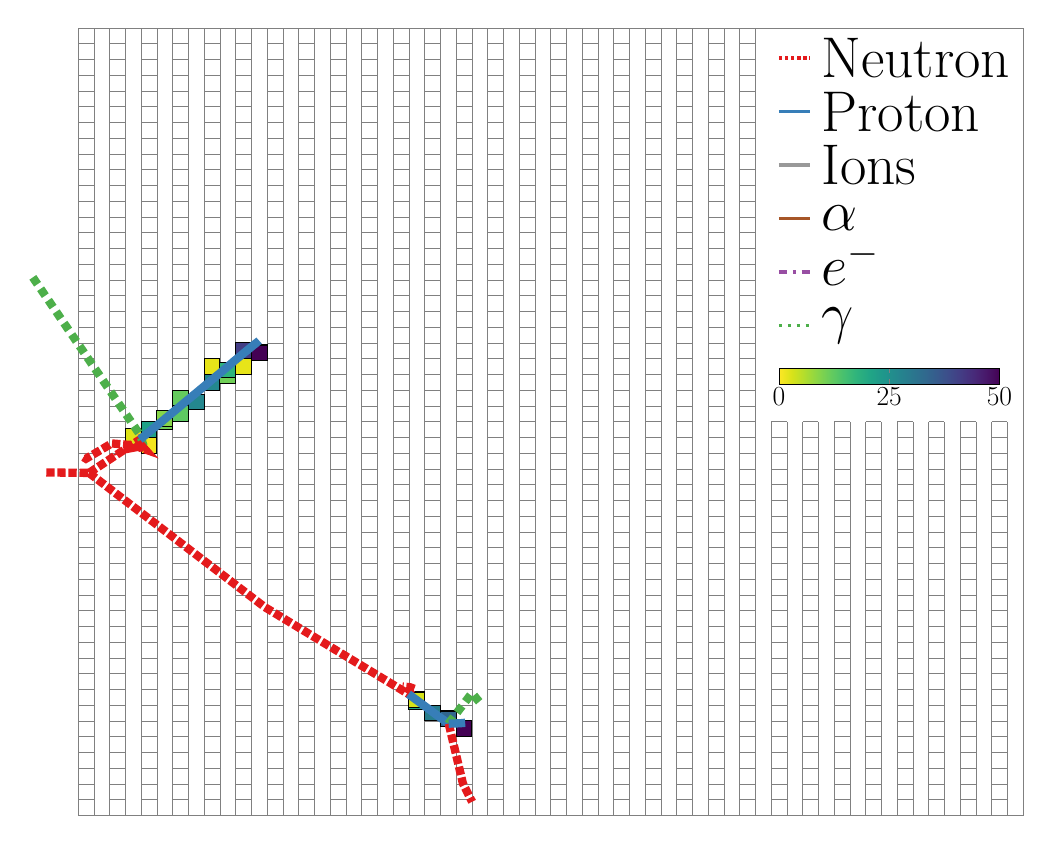
\begin{tikzpicture}[scale=0.4]
\draw[step=0.5,very thin,gray] (21.999000,-12.499) grid (22.500000,0);
\draw[step=0.5,very thin,gray] (22.999000,-12.499) grid (23.500000,0);
\draw[step=0.5,very thin,gray] (23.999000,-12.499) grid (24.500000,0);
\draw[step=0.5,very thin,gray] (24.999000,-12.499) grid (25.500000,0);
\draw[step=0.5,very thin,gray] (25.999000,-12.499) grid (26.500000,0);
\draw[step=0.5,very thin,gray] (26.999000,-12.499) grid (27.500000,0);
\draw[step=0.5,very thin,gray] (27.999000,-12.499) grid (28.500000,0);
\draw[step=0.5,very thin,gray] (28.999000,-12.499) grid (29.500000,0);
\draw[step=0.5,very thin,gray] (-0.001000,-12.499) grid (0.500000,12.499);
\draw[step=0.5,very thin,gray] (0.999000,-12.499) grid (1.500000,12.499);
\draw[step=0.5,very thin,gray] (1.999000,-12.499) grid (2.500000,12.499);
\draw[step=0.5,very thin,gray] (2.999000,-12.499) grid (3.500000,12.499);
\draw[step=0.5,very thin,gray] (3.999000,-12.499) grid (4.500000,12.499);
\draw[step=0.5,very thin,gray] (4.999000,-12.499) grid (5.500000,12.499);
\draw[step=0.5,very thin,gray] (5.999000,-12.499) grid (6.500000,12.499);
\draw[step=0.5,very thin,gray] (6.999000,-12.499) grid (7.500000,12.499);
\draw[step=0.5,very thin,gray] (7.999000,-12.499) grid (8.500000,12.499);
\draw[step=0.5,very thin,gray] (8.999000,-12.499) grid (9.500000,12.499);
\draw[step=0.5,very thin,gray] (9.999000,-12.499) grid (10.500000,12.499);
\draw[step=0.5,very thin,gray] (10.999000,-12.499) grid (11.500000,12.499);
\draw[step=0.5,very thin,gray] (11.999000,-12.499) grid (12.500000,12.499);
\draw[step=0.5,very thin,gray] (12.999000,-12.499) grid (13.500000,12.499);
\draw[step=0.5,very thin,gray] (13.999000,-12.499) grid (14.500000,12.499);
\draw[step=0.5,very thin,gray] (14.999000,-12.499) grid (15.500000,12.499);
\draw[step=0.5,very thin,gray] (15.999000,-12.499) grid (16.500000,12.499);
\draw[step=0.5,very thin,gray] (16.999000,-12.499) grid (17.500000,12.499);
\draw[step=0.5,very thin,gray] (17.999000,-12.499) grid (18.500000,12.499);
\draw[step=0.5,very thin,gray] (18.999000,-12.499) grid (19.500000,12.499);
\draw[step=0.5,very thin,gray] (19.999000,-12.499) grid (20.500000,12.499);
\draw[step=0.5,very thin,gray] (20.999000,-12.499) grid (21.500000,12.499);
\draw[very thin,gray] (0,-12.5) -- (30,-12.5) -- (30,12.5) -- (0,12.5);
\definecolor{tempcolor}{rgb}{0.866013,0.889868,0.095953}\draw[fill=tempcolor,fill opacity=1] (1.500000,-0.717350) rectangle (2.000000,-0.217350);
\definecolor{tempcolor}{rgb}{0.955300,0.901065,0.118128}\draw[fill=tempcolor,fill opacity=1] (2.000000,-1.000000) rectangle (2.500000,-0.500000);
\definecolor{tempcolor}{rgb}{0.123444,0.636809,0.528763}\draw[fill=tempcolor,fill opacity=1] (2.000000,-0.500000) rectangle (2.500000,0.000000);
\definecolor{tempcolor}{rgb}{0.449368,0.813768,0.335384}\draw[fill=tempcolor,fill opacity=1] (2.500000,-0.245136) rectangle (3.000000,0.254864);
\definecolor{tempcolor}{rgb}{0.525776,0.833491,0.288127}\draw[fill=tempcolor,fill opacity=1] (2.500000,-0.156994) rectangle (3.000000,0.343006);
\definecolor{tempcolor}{rgb}{0.369214,0.788888,0.382914}\draw[fill=tempcolor,fill opacity=1] (3.000000,0.000000) rectangle (3.500000,0.500000);
\definecolor{tempcolor}{rgb}{0.395174,0.797475,0.367757}\draw[fill=tempcolor,fill opacity=1] (3.000000,0.500000) rectangle (3.500000,1.000000);
\definecolor{tempcolor}{rgb}{0.140536,0.530132,0.555659}\draw[fill=tempcolor,fill opacity=1] (3.500000,0.373277) rectangle (4.000000,0.873277);
\definecolor{tempcolor}{rgb}{0.139147,0.533812,0.555298}\draw[fill=tempcolor,fill opacity=1] (4.000000,1.000000) rectangle (4.500000,1.500000);
\definecolor{tempcolor}{rgb}{0.906311,0.894855,0.098125}\draw[fill=tempcolor,fill opacity=1] (4.000000,1.500000) rectangle (4.500000,2.000000);
\definecolor{tempcolor}{rgb}{0.440137,0.811138,0.340967}\draw[fill=tempcolor,fill opacity=1] (4.500000,1.202253) rectangle (5.000000,1.702253);
\definecolor{tempcolor}{rgb}{0.180653,0.701402,0.488189}\draw[fill=tempcolor,fill opacity=1] (4.500000,1.392104) rectangle (5.000000,1.892104);
\definecolor{tempcolor}{rgb}{0.906311,0.894855,0.098125}\draw[fill=tempcolor,fill opacity=1] (5.000000,1.500000) rectangle (5.500000,2.000000);
\definecolor{tempcolor}{rgb}{0.262138,0.242286,0.520837}\draw[fill=tempcolor,fill opacity=1] (5.000000,2.000000) rectangle (5.500000,2.500000);
\definecolor{tempcolor}{rgb}{0.267004,0.004874,0.329415}\draw[fill=tempcolor,fill opacity=1] (5.500000,1.934886) rectangle (6.000000,2.434886);
\definecolor{tempcolor}{rgb}{0.124780,0.640461,0.527068}\draw[fill=tempcolor,fill opacity=1] (10.500000,-9.129900) rectangle (11.000000,-8.629900);
\definecolor{tempcolor}{rgb}{0.835270,0.886029,0.102646}\draw[fill=tempcolor,fill opacity=1] (10.500000,-9.084414) rectangle (11.000000,-8.584414);
\definecolor{tempcolor}{rgb}{0.154815,0.493313,0.557840}\draw[fill=tempcolor,fill opacity=1] (11.000000,-9.500000) rectangle (11.500000,-9.000000);
\definecolor{tempcolor}{rgb}{0.194100,0.399323,0.555565}\draw[fill=tempcolor,fill opacity=1] (11.500000,-9.685316) rectangle (12.000000,-9.185316);
\definecolor{tempcolor}{rgb}{0.267004,0.004874,0.329415}\draw[fill=tempcolor,fill opacity=1] (12.000000,-10.000000) rectangle (12.500000,-9.500000);
\draw[color=pdg2112, line width=3pt, densely dotted] (-1.0131056190758727, -1.6129585687041026) -- (-0.013193576250887417, -1.623783793997419) -- (0.0029999999999972713, -1.62395910852881) -- (0.34301241649914116, -1.6276401433133585);
\draw[color=pdg1000020040, line width=3pt, solid] (0.34301241649914116, -1.6276401433133585);
\draw[color=pdg1000010020, line width=3pt, solid] (0.34301241649914116, -1.6276401433133585);
\draw[color=pdg1000020040, line width=3pt, solid] (0.34301241649914116, -1.6276401433133585);
\draw[color=pdg2212, line width=3pt, solid] (0.34301241649914116, -1.6276401433133585);
\draw[color=pdg2112, line width=3pt, densely dotted] (0.34301241649914116, -1.6276401433133585) -- (0.48999999999998634, -1.7398496863895136) -- (0.7351830192832949, -1.9270211052845732) -- (0.7544915293176018, -1.9417611196233906) -- (0.7710416807755791, -1.9543954176280924) -- (0.7848334736572042, -1.9649239992986764) -- (0.9900000000000091, -2.121547039334655) -- (1.4726506626551328, -2.49) -- (1.4896798611807298, -2.503) -- (1.9899999999999864, -2.8849417452248884) -- (2.1276198367168035, -2.99) -- (2.144649035242401, -3.003) -- (2.490000000000009, -3.2666390981700326) -- (2.9899999999999864, -3.6483364511151435) -- (3.437558184840191, -3.9900000000000007) -- (3.454587383365788, -4.003) -- (3.4899999999999864, -4.030033804060272) -- (3.512850105646976, -4.047477453740212) -- (3.529400257104953, -4.0601117517449135) -- (3.5431920499865783, -4.070640333415497) -- (3.990000000000009, -4.411731157005413) -- (4.092527358901862, -4.49) -- (4.109556557427458, -4.503) -- (4.490000000000009, -4.793428509950529) -- (4.8727208837773786, -5.085595606459805) -- (4.892029393811663, -5.100335620798623) -- (4.908579545269641, -5.112969918803325) -- (4.922371338151288, -5.123498500473908) -- (4.989999999999986, -5.175125862895655) -- (5.402465707025226, -5.49) -- (5.419494905550823, -5.503) -- (5.489999999999986, -5.556823215840788) -- (5.92477343227863, -5.88872695230403) -- (5.989999999999986, -5.928183588560219) -- (6.0921899667495385, -5.989999999999999) -- (6.1037618090902015, -5.997) -- (6.113680531096475, -6.003) -- (6.121946132768381, -6.008) -- (6.489999999999986, -6.2306419091078995) -- (6.989999999999986, -6.533100229655576) -- (7.489999999999986, -6.83555855020325) -- (7.6966762714294195, -6.960580466110455) -- (7.716727073097809, -6.972709529706966) -- (7.733913474527844, -6.983105869932547) -- (7.748235475719548, -6.991769486787199) -- (7.989999999999986, -7.138016870750934) -- (8.489999999999986, -7.44047519129861) -- (8.989999999999986, -7.742933511846286) -- (9.39843063551093, -7.99) -- (9.410002477851595, -7.997) -- (9.419921199857868, -8.003) -- (9.428186801529773, -8.008) -- (9.489999999999986, -8.04539183239398) -- (9.989999999999986, -8.347850152941657) -- (10.224990802701246, -8.49) -- (10.236562645041886, -8.497) -- (10.246481367048181, -8.503) -- (10.254746968720065, -8.508) -- (10.4868686382546, -8.648414260660271) -- (10.497000000000025, -8.630232891805566) -- (10.502999999999997, -8.619465512664531) -- (10.510084424295655, -8.606752065599938) -- (10.514317412146397, -8.599155701418546) -- (10.548206963963912, -8.538338759195225) -- (10.58935035824852, -8.4875965683453) -- (10.609739999817133, -8.470730101393952) -- (10.679795365373753, -8.484914686462982) -- (10.53165254417038, -8.431237796086982) -- (10.510000000000014, -8.429102570886677) -- (10.295392883833006, -8.40793949097334);
\draw[color=pdg2212, line width=3pt, solid] (10.609739999817133, -8.470730101393952);
\draw[color=pdg2212, line width=3pt, solid] (10.548206963963912, -8.538338759195225);
\draw[color=pdg2212, line width=3pt, solid] (10.4868686382546, -8.648414260660271) -- (10.576688123058101, -8.715585432220289) -- (10.601033411674234, -8.733726965502747) -- (10.622337615340347, -8.749580731718916) -- (10.64009111839548, -8.762792203565724) -- (10.990000000000009, -9.020886547683267) -- (11.446544073320501, -9.361436391607635) -- (11.489999999999986, -9.392538617207721) -- (11.763699017662157, -9.588059002297523);
\draw[color=pdg1000060110, line width=3pt, solid] (11.763699017662157, -9.588059002297523);
\draw[color=pdg22, line width=3pt, dotted] (11.763699017662157, -9.588059002297523) -- (11.7741711319994, -9.567265316933256) -- (11.990000000000009, -9.285537155490704) -- (12.002999999999997, -9.268567849518446) -- (12.201086005946877, -9.01) -- (12.489999999999986, -8.632871541172229) -- (12.502999999999997, -8.615902235199941) -- (12.663883534618957, -8.811387669438847) -- (12.679364931085093, -8.829573078911537) -- (12.692634699484643, -8.84516057274527) -- (12.703692839817586, -8.858150150940048) -- (12.794370391629059, -8.964665633136978) -- (12.807111591283501, -8.971521517544879);
\draw[color=pdg11, line width=3pt, dashdotted] (12.807111591283501, -8.971521517544879);
\draw[color=pdg11, line width=3pt, dashdotted] (12.794370391629059, -8.964665633136978);
\draw[color=pdg11, line width=3pt, dashdotted] (12.49330496902851, -8.611015495694005);
\draw[color=pdg11, line width=3pt, dashdotted] (12.515126061812634, -8.600073708035515);
\draw[color=pdg11, line width=3pt, dashdotted] (11.7741711319994, -9.567265316933256);
\draw[color=pdg2112, line width=3pt, densely dotted] (11.763699017662157, -9.588059002297523) -- (11.97149392135941, -10.462731244978226) -- (11.976530716083493, -10.483932652995714) -- (11.980847968704143, -10.502105288439276) -- (11.984445679221334, -10.517249151308912) -- (11.989999999999986, -10.540628984623348) -- (11.99699999999998, -10.570094123516661) -- (12.002999999999997, -10.595349956853862) -- (12.007999999999992, -10.6163964846348) -- (12.096756568126967, -10.99) -- (12.21554100734752, -11.49) -- (12.467699250833197, -11.99) -- (12.489999999999986, -12.034126964648717) -- (12.497000000000025, -12.047978012890713) -- (12.502999999999997, -12.05985033995521) -- (12.507999999999992, -12.06974394584234);
\draw[color=pdg2212, line width=3pt, solid] (11.763699017662157, -9.588059002297523) -- (11.878168849188887, -9.58602280126819) -- (11.968799928495718, -9.58268453511571) -- (11.989999999999986, -9.581660204290023) -- (12.074602846647645, -9.578313799827793) -- (12.1261957350265, -9.57581883405266) -- (12.16712850050617, -9.572168683382698) -- (12.199691612920379, -9.56837959794952) -- (12.226146939702108, -9.566141667407411) -- (12.246985940003174, -9.564801801980044) -- (12.263507026680987, -9.56347118975001) -- (12.276721463944956, -9.56225692194932) -- (12.287391917471997, -9.561469577175302);
\draw[color=pdg2112, line width=3pt, densely dotted] (0.34301241649914116, -1.6276401433133585) -- (0.48999999999998634, -1.5311454465504997) -- (0.9900000000000091, -1.2029044670588727) -- (1.2838458009686065, -1.0100000000000002) -- (1.303648325351969, -0.9970000000000001) -- (1.490000000000009, -0.874663487567253) -- (1.9613852304058128, -0.5652075880746661) -- (1.990000000000009, -0.6173179015473776) -- (1.9970000000000028, -0.6300655909218327) -- (2.0029999999999974, -0.6409921818142412) -- (2.007999999999993, -0.6500976742245912) -- (2.0720017007206026, -0.76665107425667);
\draw[color=pdg22, line width=3pt, dotted] (2.0720017007206026, -0.76665107425667) -- (2.0100000000000136, -0.5493721848706129) -- (2.0029999999999744, -0.5248413702634537) -- (1.9970000000000028, -0.5038149577431505) -- (1.9920000000000073, -0.48629294730947814) -- (1.979750747155458, -0.44336664008016646) -- (1.8147555684805865, -0.20095705111789286) -- (1.570612545863537, 0.15773591334273254) -- (1.509999999999991, 0.24678737803848771) -- (1.5029999999999972, 0.25707172171666154) -- (1.4970000000000028, 0.2658868734408226) -- (1.4920000000000073, 0.27323283321096525) -- (1.3444582399223237, 0.49000000000000005) -- (1.3356098386195527, 0.5030000000000001) -- (1.009999999999991, 0.9813833550516904) -- (1.0029999999999972, 0.9916676987298642) -- (0.9970000000000028, 1.000482850454025) -- (0.9920000000000073, 1.007828810224168) -- (0.8381834780124336, 1.2338148067246082) -- (0.5940404553954067, 1.5925077711852333) -- (0.5099999999999909, 1.7159793320648369) -- (0.5029999999999972, 1.7262636757430108) -- (0.4970000000000027, 1.7350788274671718) -- (0.49200000000000726, 1.7424247872373144) -- (0.3234888588355034, 1.9899999999999998) -- (0.3146404575327324, 2.0029999999999997) -- (0.010000000000013642, 2.4505753090780202) -- (0.0029999999999745343, 2.4608596527562274) -- (-0.3657866573752699, 3.0026780425242596) -- (-0.7345733147505371, 3.5444964322922923) -- (-1.1033599721257814, 4.086314822060325) -- (-1.4721466295010486, 4.628133211828358);
\draw[color=pdg11, line width=3pt, dashdotted] (1.979750747155458, -0.44336664008016646) -- (1.9841796244770649, -0.43531050956711964);
\draw[color=pdg1000060120, line width=3pt, solid] (2.0720017007206026, -0.76665107425667);
\draw[color=pdg2112, line width=3pt, densely dotted] (2.0720017007206026, -0.76665107425667) -- (2.0100000000000136, -0.7784407732761233) -- (1.9783962916499376, -0.7844502569679481) -- (1.8421734803943537, -0.8103531906878535) -- (1.9899999999999864, -0.7320064715236103) -- (2.1204779133097644, -0.8795492374359964) -- (2.009999999999991, -0.8411262473701285) -- (1.7398770568614963, -0.7471804907040677) -- (1.509999999999991, -0.7283381610133557) -- (1.0639050268693837, -0.6917731002288828) -- (1.0100000000000136, -0.7237994582035369) -- (0.6486489251678677, -0.938487392691386) -- (0.5100000000000137, -1.0208622725145005) -- (0.24713470859708195, -1.1770372790121448) -- (0.1185857509238076, -1.0967579920952804);
\draw[color=pdg2212, line width=3pt, solid] (0.24713470859708195, -1.1770372790121448);
\draw[color=pdg2212, line width=3pt, solid] (1.0639050268693837, -0.6917731002288828);
\draw[color=pdg1000060120, line width=3pt, solid] (2.1204779133097644, -0.8795492374359964);
\draw[color=pdg1000060120, line width=3pt, solid] (2.0143396841896903, -0.7191066589132461);
\draw[color=pdg1000060120, line width=3pt, solid] (1.8421734803943537, -0.8103531906878535);
\draw[color=pdg2212, line width=3pt, solid] (1.9613852304058128, -0.5652075880746661) -- (1.990000000000009, -0.5414780615496133) -- (2.0283455580208285, -0.51) -- (2.4899999999999864, -0.12888992628850732) -- (2.725095660431566, 0.06466351736477097) -- (2.7508631861584716, 0.08593429114808156) -- (2.7727073371542246, 0.10401525315009721) -- (2.790910796317371, 0.11908272148511063) -- (2.990000000000009, 0.284742972364534) -- (3.2364717855957226, 0.49000000000000005) -- (3.4899999999999864, 0.6997868773733795) -- (3.9644502681315315, 1.0927786681399192) -- (3.990000000000009, 1.1140593798526637) -- (4.361284818872468, 1.426377468962516) -- (4.438467167970794, 1.49) -- (4.490000000000009, 1.532531031636383) -- (4.6626437951576465, 1.6772932088107406) -- (4.67213810990736, 1.6852471667731108) -- (4.6959831254633855, 1.7051179043009246) -- (4.724107412451849, 1.7292101561198556) -- (4.747544318275596, 1.7492870326356307) -- (4.757219299147527, 1.7576025773274122) -- (4.959849297071196, 1.9309861767267744) -- (4.989999999999986, 1.9557230941725028) -- (5.031938303327979, 1.9899999999999998) -- (5.203355135821971, 2.130342167524479) -- (5.320695651277697, 2.2280575821274153) -- (5.414155137301532, 2.3037176158650823) -- (5.488232979288091, 2.3641036331281695) -- (5.564983445239409, 2.4269816937297084) -- (5.608959409970771, 2.461926937902575) -- (5.643637692212747, 2.489549741098082) -- (5.671365708972099, 2.5118666290335745) -- (5.693425965059214, 2.529511298677269) -- (5.7109125475960125, 2.5438854306890635) -- (5.7247449338138265, 2.5557586190991612) -- (5.735640543199224, 2.5653027472980354) -- (5.744261765843521, 2.5730292116268245);
\draw[color=pdg2112, very thick, densely dotted] (22.25,11.550000) -- (23.25,11.550000) node [right,black] {\huge{Neutron}};
\draw[color=pdg2212, very thick, solid] (22.25,9.850000) -- (23.25,9.850000) node [right,black] {\huge{Proton}};
\draw[color=pdg1000010020, very thick, solid] (22.25,8.150000) -- (23.25,8.150000) node [right,black] {\huge{Ions}};
\draw[color=pdg1000020040, very thick, solid] (22.25,6.450000) -- (23.25,6.450000) node [right,black] {\huge{$\alpha$}};
\draw[color=pdg11, very thick, dashdotted] (22.25,4.750000) -- (23.25,4.750000) node [right,black] {\huge{$e^-_{\vphantom{-}}$}};
\draw[color=pdg22, very thick, dotted] (22.25,3.050000) -- (23.25,3.050000) node [right,black] {\huge{$\gamma$}};
\begin{axis}[%
    at={(22.25cm,2cm)}, %4.75
    hide axis,
    scale only axis,
    height=0pt,
    width=0pt,
    colormap={reverse viridis}{
       indices of colormap={
       \pgfplotscolormaplastindexof{viridis},...,0 of viridis}
    },
    colorbar horizontal,
    point meta min=0,
    point meta max=50,
    label style={font=\Huge},
    tick label style={font=\Huge},
    colorbar style={
       width=7cm,
       xtick={50, 25, 0},
    }]
\end{axis}
\end{tikzpicture}
\end{document}
